\section{Wyniki i analiza badań}
To co wyszło i jak

\subsection{Rekonstrukcja}

\subsubsection{Gaussian Splatting}
Jak już wcześniej zostało wspomniane, algorytm posiada wiele hiperparametrów które mogą mieć różne optymalne wartości w zależności od sceny. Ogólnym więc zaleceniem jest uruchomienie algorytmu dla różnych wartości, a za pomoc mogą posłużyć poniższe wyniki naszych badań. 

Uwaga: do renderowania została użyta funkcjonalność biblioteki gsplat, więc wyniki mogą się różnić dla naszego własnego renderowania. 


\textbf{Eksperymenty dla sceny SKS}

Poniżej zostaną opisane wyniki różnych trenowań dla sceny SKS. 

\begin{table}[h]
    \centering
    \begin{tabular}{|c|c|c|c|c|c|c|c|c|c|}
    \hline
    i & init\_opa & init\_scale & init\_type & scale\_reg & sh\_degree & sh\_interval & strategy & cap\_max & refine\_every \\
    \hline
    14 & 0.10 & 1.00 & sfm & 0.00 & 3 & 5000 & default & nan & 100 \\
    \hline
    15 & 0.10 & 1.00 & sfm & 0.01 & 3 & 5000 & default & nan & 100 \\
    \hline
    16 & 0.10 & 1.00 & sfm & 0.01 & 3 & 5000 & default & nan & 500 \\
    \hline
    17 & 0.10 & 1.00 & sfm & 0.01 & 3 & 5000 & default & nan & 1000 \\
    \hline
    18 & 0.50 & 0.10 & sfm & 0.01 & 3 & 5000 & default & nan & 1000 \\
    \hline
    19 & 0.10 & 1.00 & sfm & 0.01 & 3 & 5000 & mcmc & 3000000.00 & 100 \\
    \hline
    20 & 0.10 & 1.00 & sfm & 0.01 & 3 & 5000 & mcmc & 3000000.00 & 500 \\
    \hline
    21 & 0.10 & 1.00 & sfm & 0.01 & 3 & 5000 & mcmc & 3000000.00 & 1000 \\
    \hline
    22 & 0.50 & 0.10 & sfm & 0.01 & 3 & 5000 & mcmc & 3000000.00 & 100 \\
    \hline
    23 & 0.50 & 0.10 & sfm & 0.01 & 1 & 5000 & mcmc & 3000000.00 & 100 \\
    \hline
    \end{tabular}
    \caption{Konfiguracja trenowania dla sceny SKS}
    \label{table:tab_conf_sks}
\end{table}

W powyższej tabeli \ref{table:tab_conf_sks} uwzględnione są najważniejsze hiperparametry od których zależy jakość trenowania i końcowych wyników. 

\begin{table}[h]
    \centering
    \begin{tabular}{|c|c|c|c|c|c|c|c|}
    \hline
    i & iteration & psnr & ssim & lpips & num\_GS & time & size (MB) \\
    \hline
    14 & 19900.00 & 20.64 & 0.65 & 0.44 & 3268771.00 & 17475.92 & 735.00 \\
    \hline
    15 & 11500.00 & 19.75 & 0.59 & 0.59 & 2825402.00 & 7222.10 & 635.00 \\
    \hline
    16 & 46500.00 & 21.77 & 0.70 & 0.29 & 3685999.00 & 17008.88 & 829.00 \\
    \hline
    17 & 71999.00 & 21.81 & 0.71 & 0.25 & 3286360.00 & 20822.40 & 739.00 \\
    \hline
    18 & 63200.00 & 22.04 & 0.71 & 0.25 & 2937549.00 & 10357.16 & 661.00 \\
    \hline
    19 & 56999.00 & 22.35 & 0.71 & 0.24 & 3000000.00 & 28671.98 & 675.00 \\
    \hline
    20 & 41999.00 & 21.65 & 0.70 & 0.32 & 2699815.00 & 14345.60 & 607.00 \\
    \hline
    21 & 89499.00 & 20.83 & 0.67 & 0.38 & 3000000.00 & 37661.22 & 675.00 \\
    \hline
    22 & 31999.00 & 21.59 & 0.68 & 0.37 & 3000000.00 & 33266.17 & 675.00 \\
    \hline
    23 & 44499.00 & 21.29 & 0.69 & 0.29 & 3000000.00 & 17769.49 & 263.00 \\
    \hline
    \end{tabular}
    \caption{Wyniki eksperymentów dla sceny SKS}
    \label{table:tab_res_sks}
\end{table}

\begin{figure}[!h]
    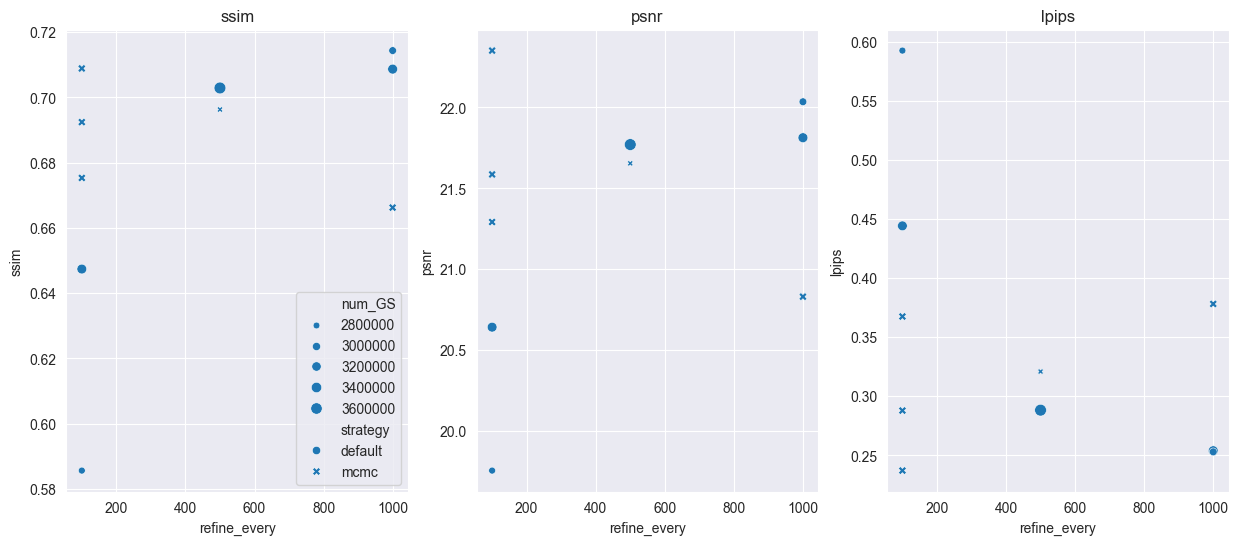
\includegraphics[width=\linewidth]{img/metrics_1.png}
    \caption{B}\label{fig:metrics_1}
\end{figure}

\begin{figure}[!h]
    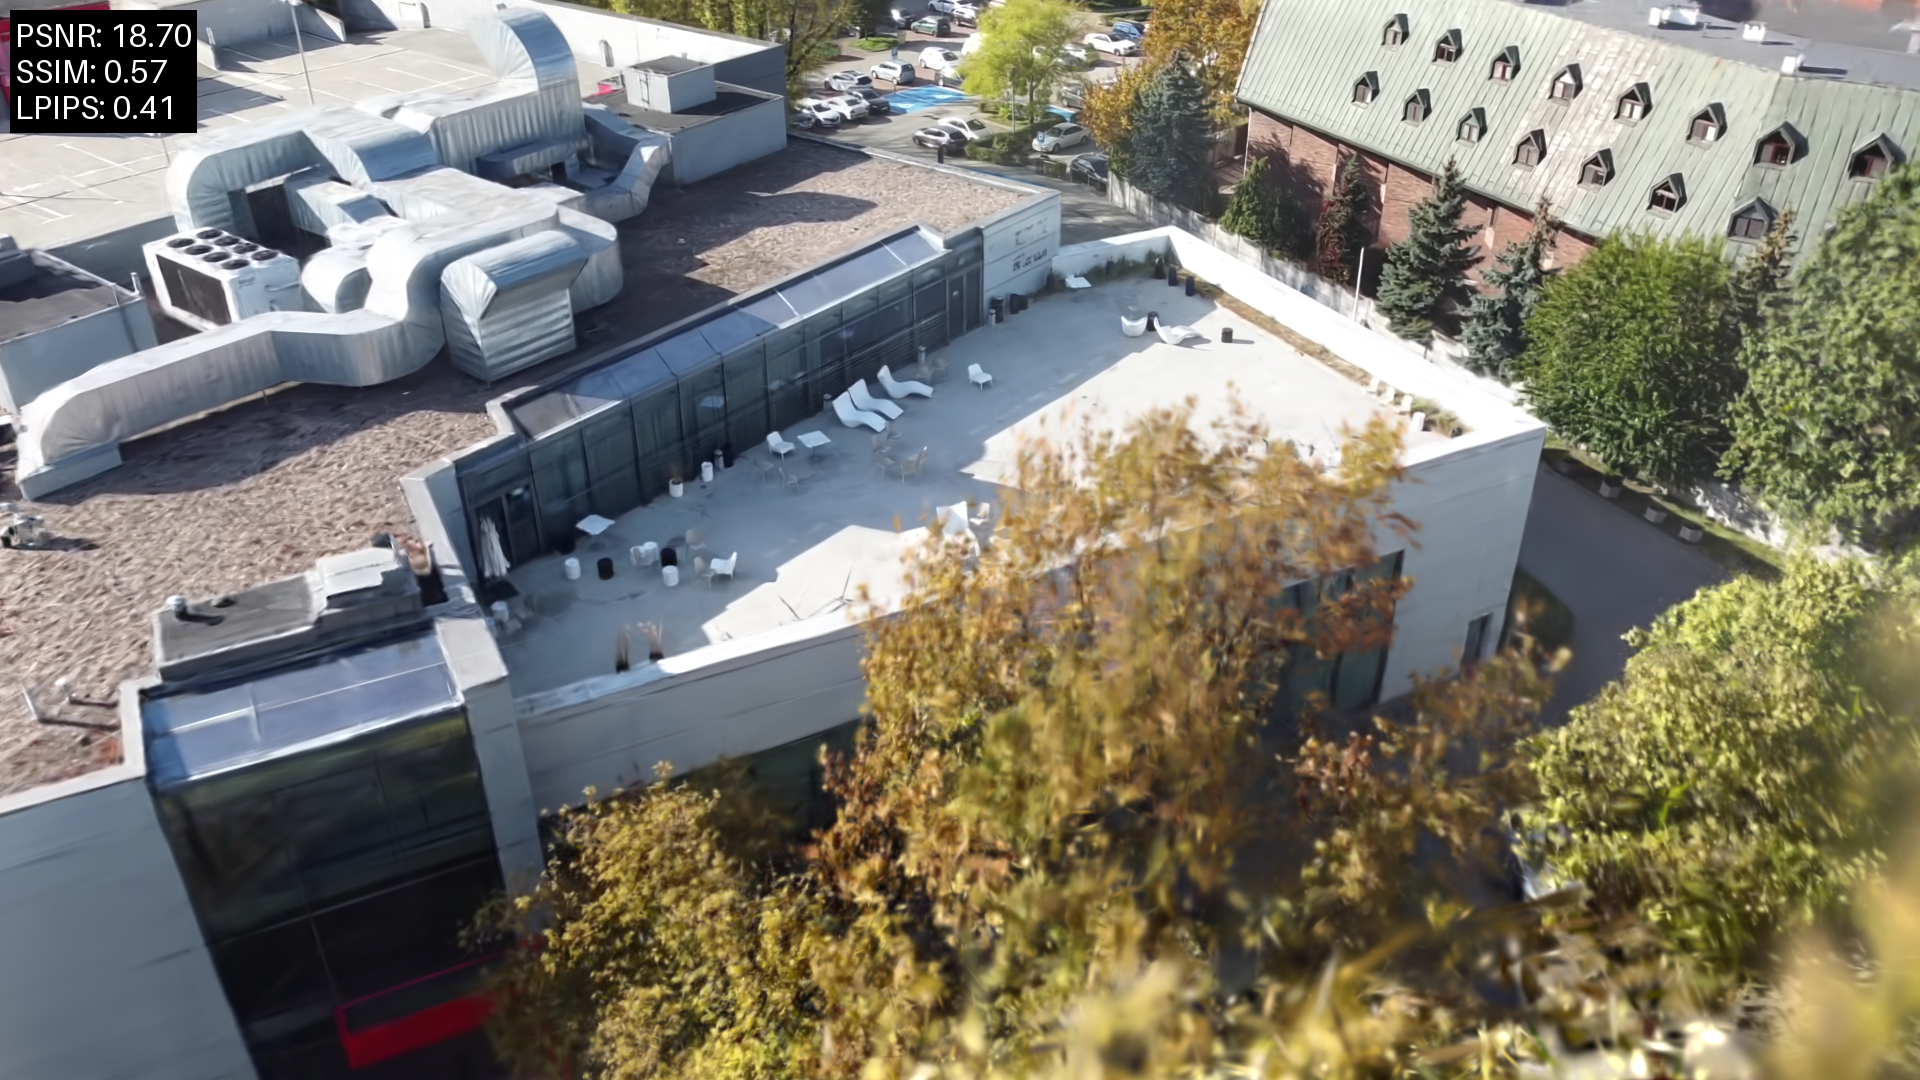
\includegraphics[width=\linewidth]{img/res_imgs/eval_with_metrics_0010_14.png}
    \caption{A}\label{fig:eval_14}
\end{figure}
